\section{Actividad 1: Corriente de Saturación $I_{DSS}$}

\subsection{Simulación}

Para la primera simulacion vamos a implementar el siguiente circuito al simulador (LTSpice).
Resaltamos que en nuestro caso usamos el JFET MPF102, por lo cual añadimos una resistencia al drenador para proteger el elemento, dicha resistencia es de 510$\Omega$. Por lo que la añadiremos de ahora en adelante a las simulaciones para ser mas precisas.

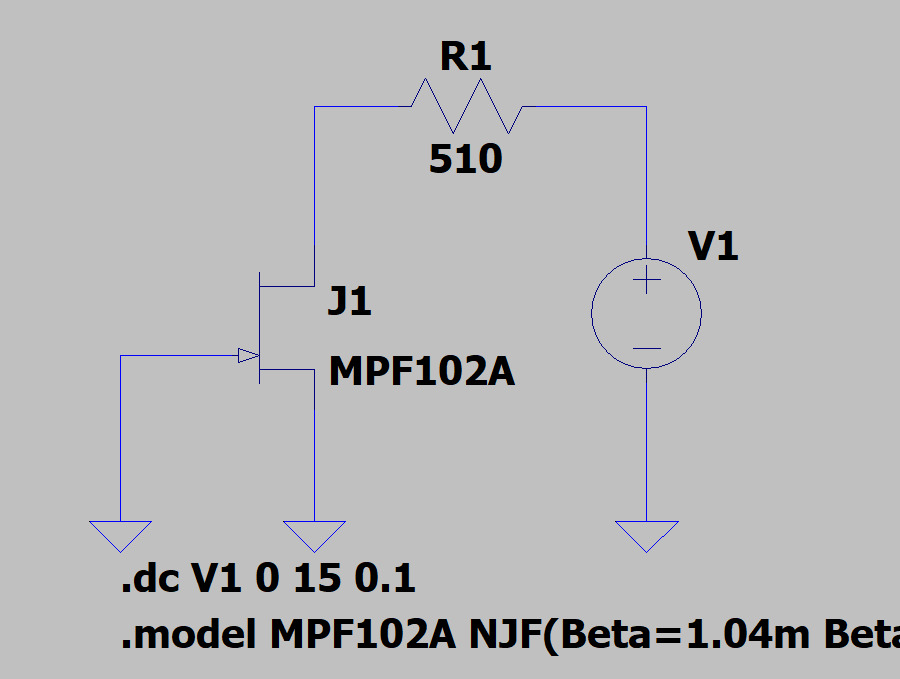
\includegraphics[width=6cm]{./imagenes/Circ1.png}

Observando el comportamiento de $I_{DS}$ con respecto a $V_{DS}$, obtenemos la siguiente gráfica:

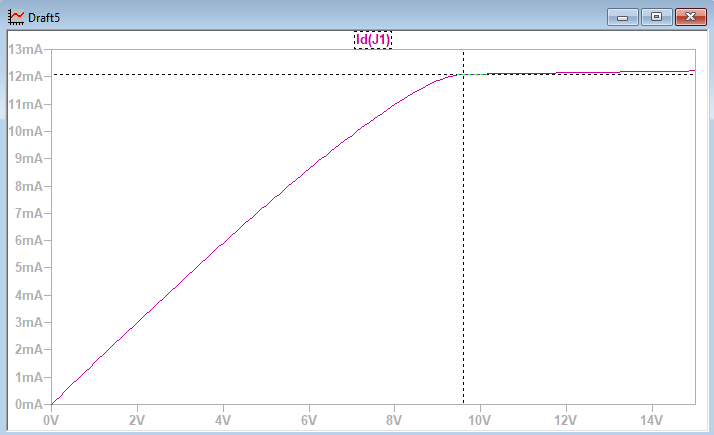
\includegraphics[width=8cm]{./imagenes/Sim1.png}

\subsection{Laboratorio}

\paragraph{Instrumental y Materiales}
\begin{itemize}
    \item Multimetro UNI-T UT89X
    \item Transistor JFET MPF102
    \item Resistor de 510$\Omega$
    \item Fuente de alimentación
\end{itemize}

\paragraph{Procedimiento:}

Para la realizacion de la actividad implementamos el circuito mostrado en la siguiente imagen, e hicimos variar el voltaje de la fuente desde 0 hasta 15V, punto en el que consideramos que el JFET mantiene su corriente constante. Los saltos medidos fueron impresisos para ver que ocurria en cada nivel de voltaje distinto hasta llegar a los 15V mencionados anteriormente.


Ejemplo de medición a 3V:

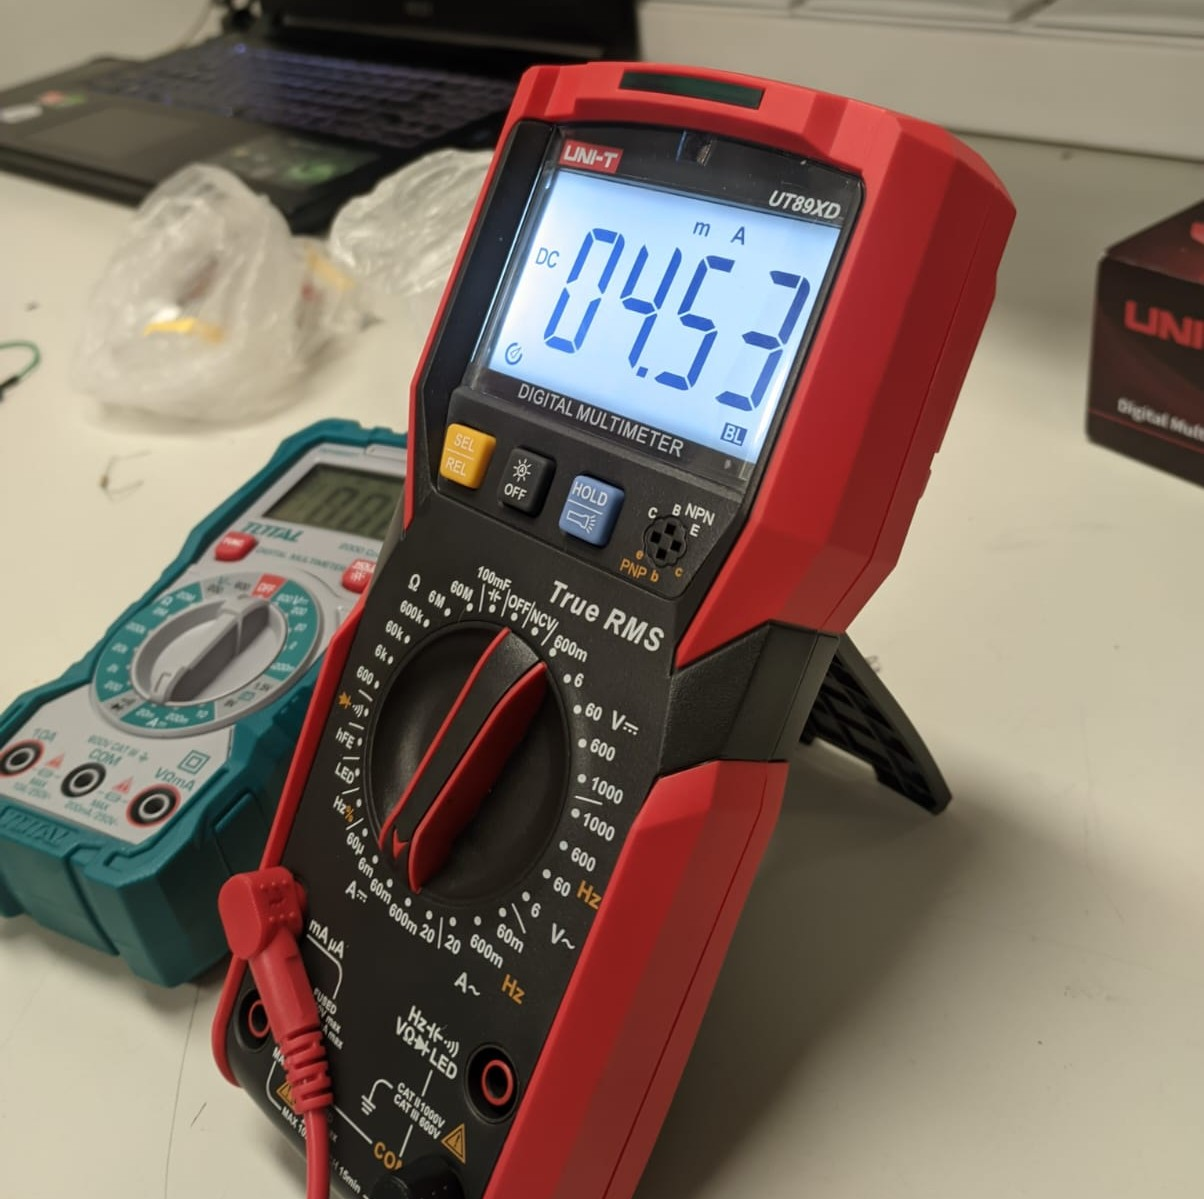
\includegraphics[width=6cm]{./imagenes/Res1.jpg}

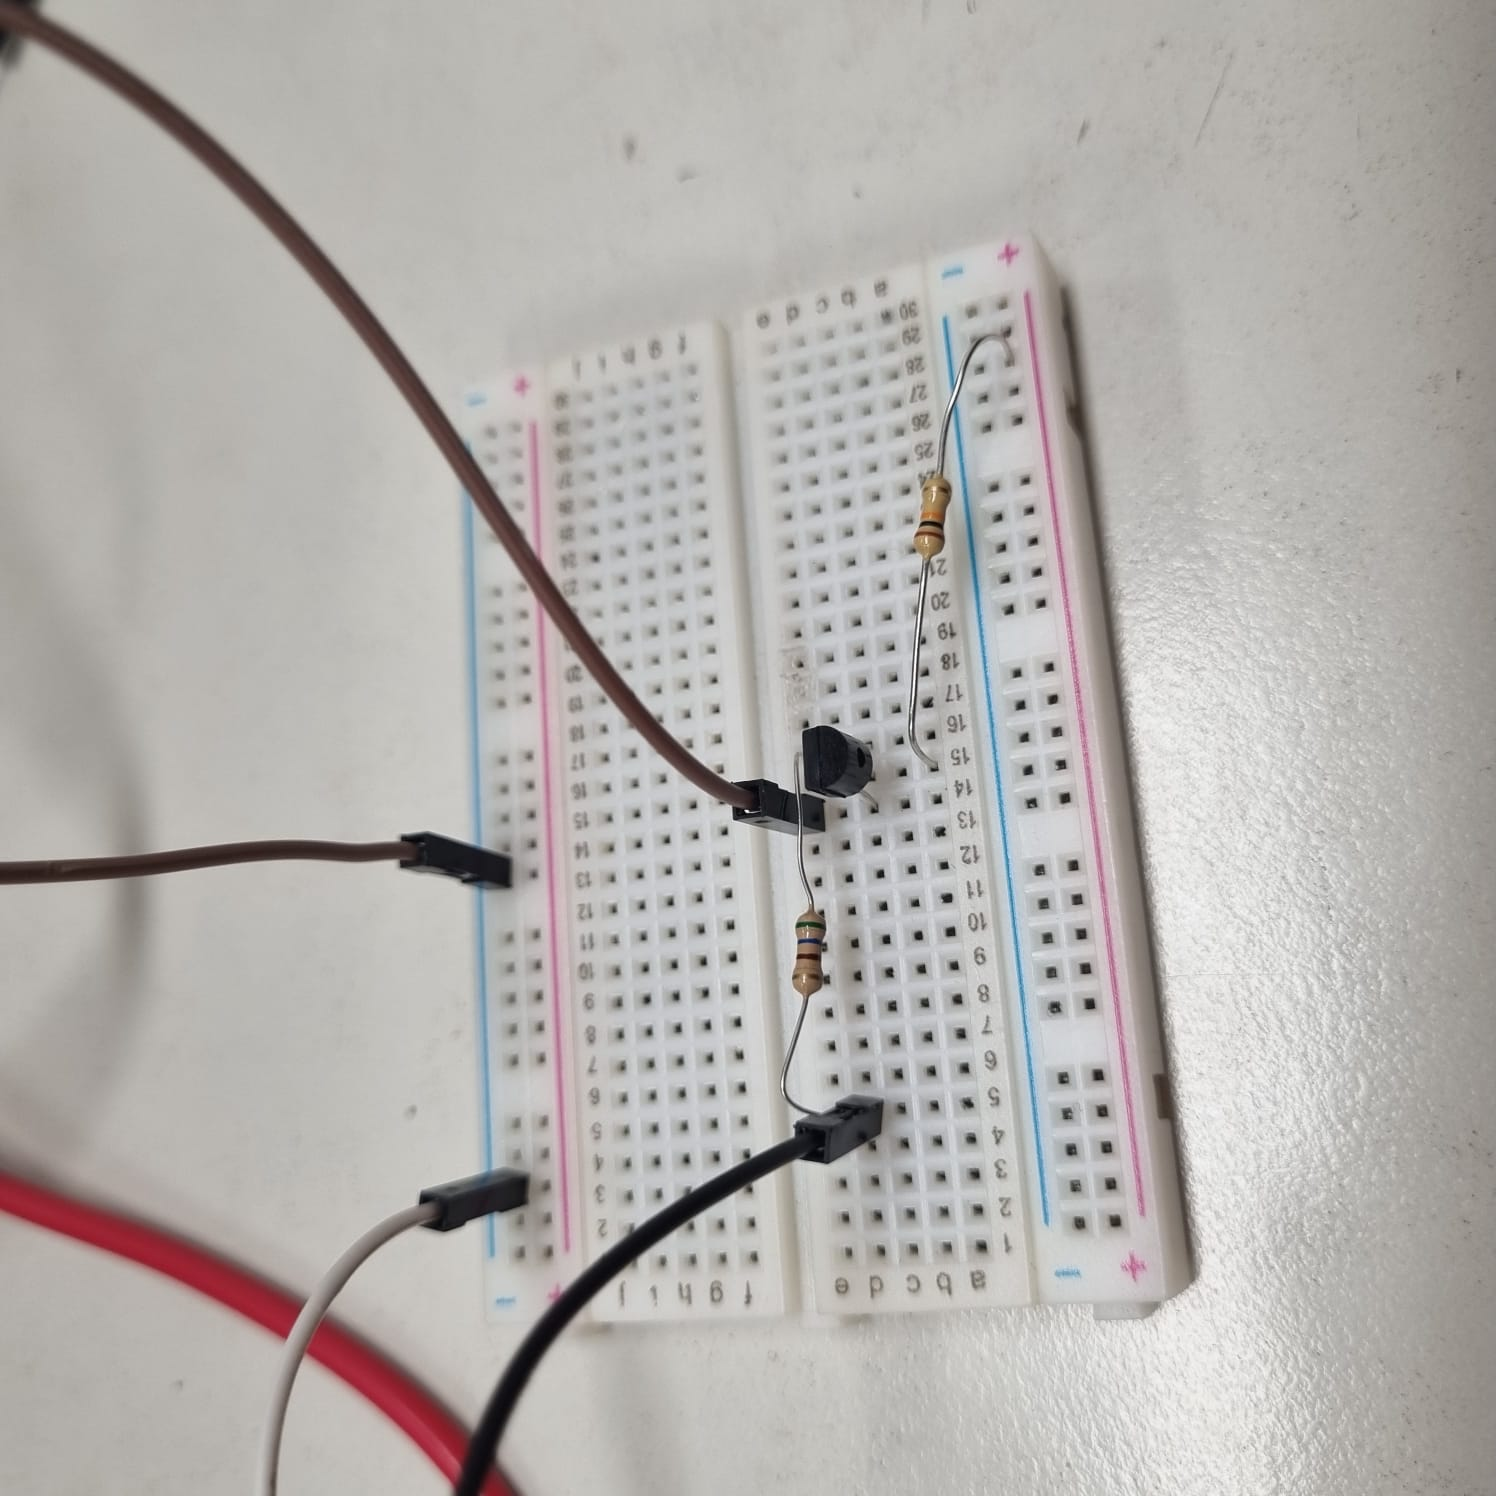
\includegraphics[width=6cm]{./imagenes/Lab1.jpg}


\begin{table}[ht]
\resizebox{4.5cm}{!}{%
\begin{tabular}{|l|l|}
\hline
\rowcolor[HTML]{FFCE93} 
$V_{DS}$ & $I_D$     \\ \hline
$150mV$  & $0,210mA$ \\ \hline
$1V$     & $1,61mA$  \\ \hline
$1,5V$   & $2,43mA$  \\ \hline
$2V$     & $3,2mA$   \\ \hline
$4V$     & $5,36mA$  \\ \hline
$6V$     & $6,48mA$  \\ \hline
$8V$     & $7,34mA$  \\ \hline
$10V$    & $8mA$     \\ \hline
$14,8V$  & $9,56mA$  \\ \hline
\end{tabular}
}
\end{table}

\vspace{0.1cm}

\begin{figure}[ht]
    \centering
    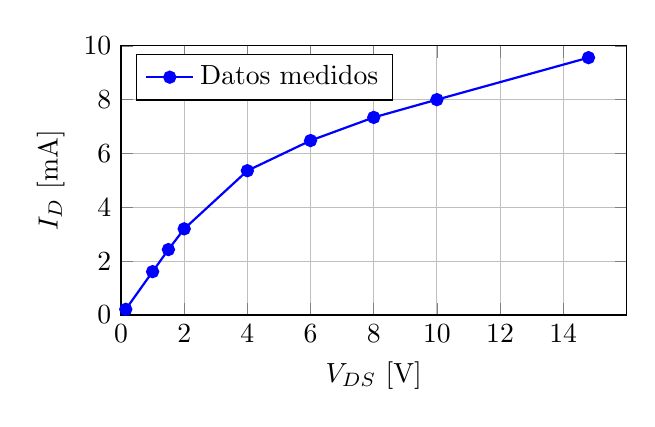
\begin{tikzpicture}
        \begin{axis}[
            width=8cm,
            height=5cm,
            xlabel={$V_{DS}$ [V]},
            ylabel={$I_D$ [mA]},
            grid=major,
            ymin=0, ymax=10,
            xmin=0, xmax=16,
            xtick={0,2,4,6,8,10,12,14},
            ytick={0,2,4,6,8,10},
            legend pos=north west
        ]
        \addplot[
            color=blue,
            mark=*,
            thick
        ] coordinates {
            (0.15,0.210)
            (1,1.61)
            (1.5,2.43)
            (2,3.2)
            (4,5.36)
            (6,6.48)
            (8,7.34)
            (10,8)
            (14.8,9.56)
        };
        \legend{Datos medidos}
        \end{axis}
    \end{tikzpicture}
    \caption{Gráfica de $I_D$ vs $V_{DS}$ obtenida en laboratorio}
\end{figure}


\subsection{Conclusión}

Podemos ver que el valor de $I_{DSS}$ es 9,56, lo cual difiere con el obtenido en la hoja de datos el cual es de 20mA, pero esto se debe a dos factores.\\
El primero es que la calidad del JFET seleccionado no es muy buena, y por ello hay diferencias en los valores.\\
Y la segunda es que para proteccion del elemento se le añadio la resistencia mencionada anteriormente, lo cual hace menor la corriente de drenaje.

\section{Actividad 2: Estrangulamiento del Canal $V_{GS(off)}$}

\subsection{Simulación}

Para la siguente simulacion añadiremos una fuente que varía de 0 a 7 en polarizaión inversa a la compuerta para extrangular el canal, obteniendo el siguiente circuito:

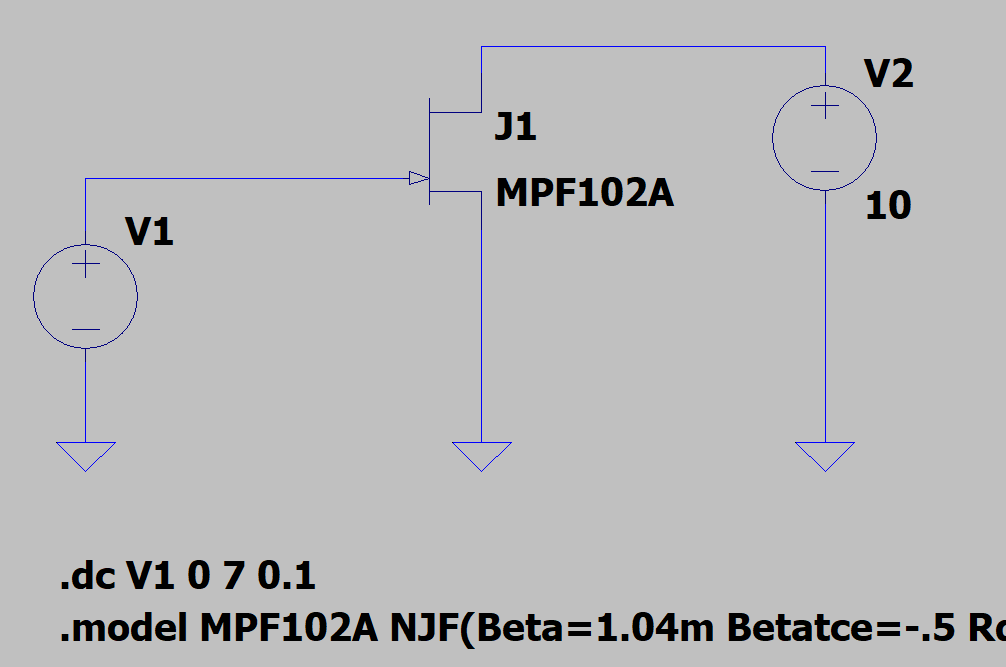
\includegraphics[width=6cm]{./imagenes/Circ2.png}

Al simularlo se obtiene la siguiente gráfica:
\begin{figure}[ht]
    \centering
    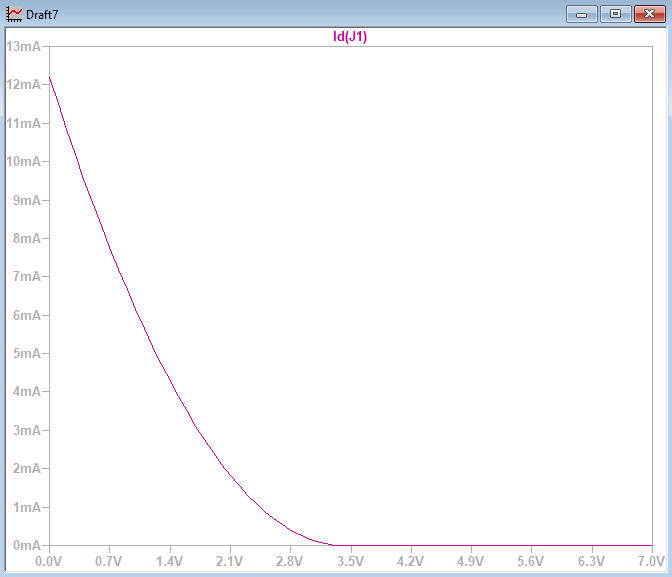
\includegraphics[width=8cm]{./imagenes/Sim2.png}
    \caption{Gráfica de $I_D$ (mA) vs $V_{GS}$ (V) obtenida en simulación}
    \label{fig:sim2}
\end{figure}

En ella observamos El valor $I_{DSS}$ de la simulación anterios rondando los 12mV, y ademas obtenemos un nuevo valor, el cual es $V_{GS(off)}$ que en nuestro caso es de -3,3V.

\subsection{Laboratorio}

\paragraph{Instrumental y Materiales}
\begin{itemize}
    \item Multimetro UNI-T UT89X
    \item Transistor JFET MPF102
    \item Resistores de 470$\Omega$ y 550$\Omega$
    \item Fuente de alimentación
\end{itemize}

\paragraph{Procedimiento}

Para dicha actividad implementamos el circuito mostrado en la siguiente imagen, usando dos fuentes dejamos la vuente $V_{DS}$ en 15V, y variamos lentamente la fuente $V_{GS}$ en polarización inversa hasta que la corriente $I_D$ sea 0.

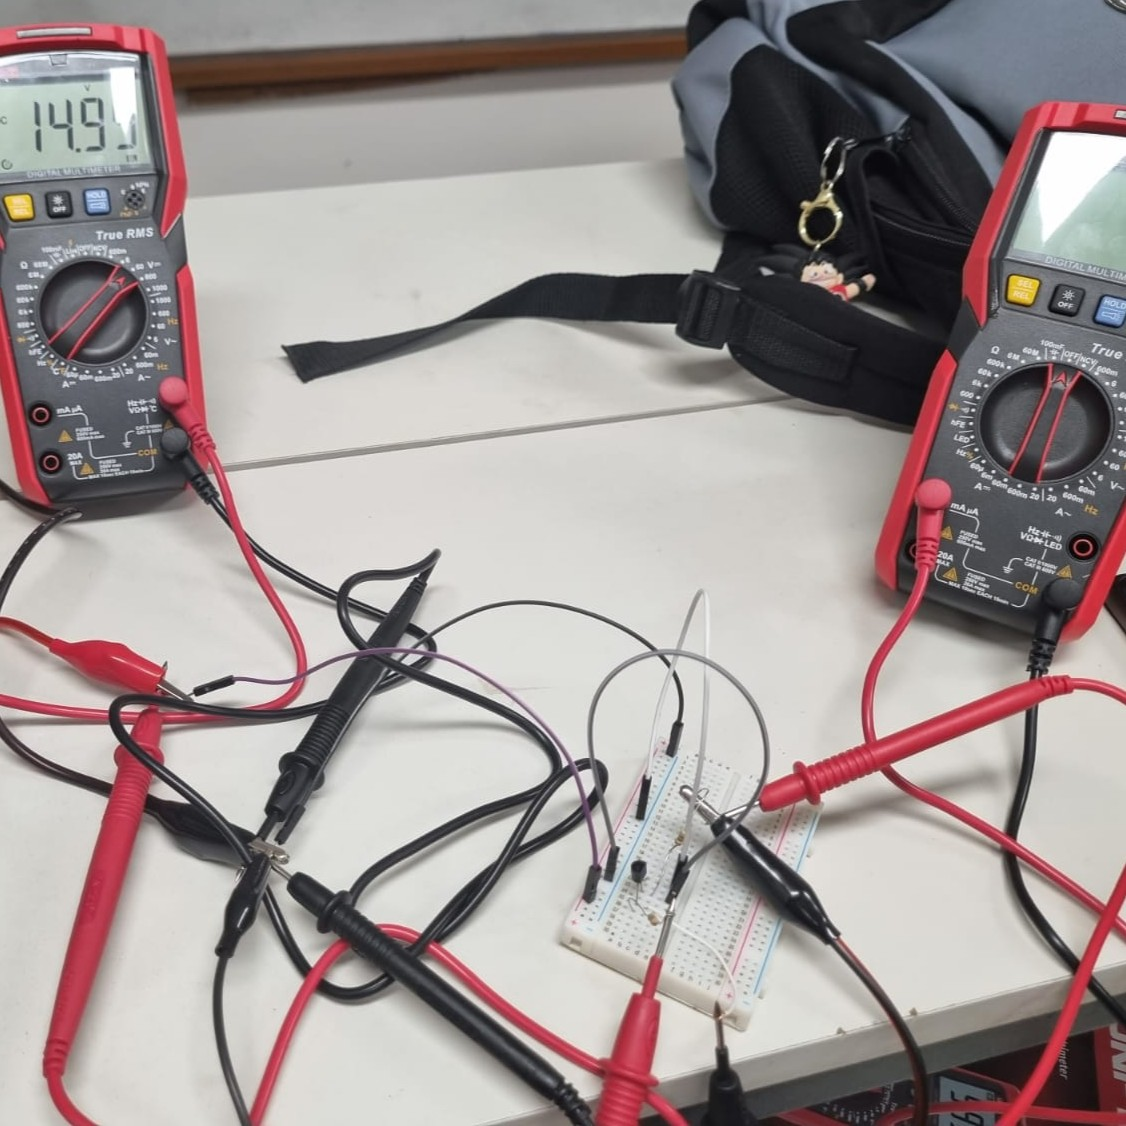
\includegraphics[width=6cm]{./imagenes/Lab2.jpg}

\begin{table}[ht]
\resizebox{5cm}{!}{%
\begin{tabular}{|l|l|}
\hline
\rowcolor[HTML]{FFCC67} 
$V_{GS}${[}mV{]} & $I_D${[}mA{]} \\ \hline
0                & 9,17          \\ \hline
36               & 8,57          \\ \hline
96,5             & 5,61          \\ \hline
172              & 4,06          \\ \hline
230              & 2,78          \\ \hline
265              & 2,46          \\ \hline
348              & 1,36          \\ \hline
396              & 0,86          \\ \hline
451              & 0,49          \\ \hline
537              & 0,21          \\ \hline
700              & 0,00124       \\ \hline
\end{tabular}%
}
\end{table}

\vspace{0.1cm}

\begin{figure}[ht]
    \centering
    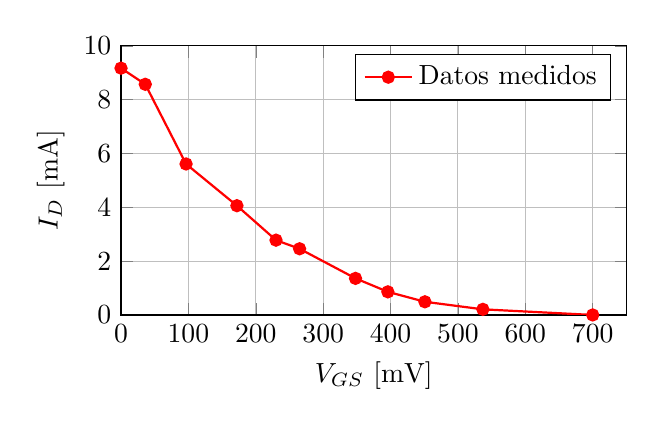
\begin{tikzpicture}
        \begin{axis}[
            width=8cm,
            height=5cm,
            xlabel={$V_{GS}$ [mV]},
            ylabel={$I_D$ [mA]},
            grid=major,
            ymin=0, ymax=10,
            xmin=0, xmax=750,
            xtick={0,100,200,300,400,500,600,700},
            ytick={0,2,4,6,8,10},
            legend pos=north east
        ]
        \addplot[
            color=red,
            mark=*,
            thick
        ] coordinates {
            (0,9.17)
            (36,8.57)
            (96.5,5.61)
            (172,4.06)
            (230,2.78)
            (265,2.46)
            (348,1.36)
            (396,0.86)
            (451,0.49)
            (537,0.21)
            (700,0.00124)
        };
        \legend{Datos medidos}
        \end{axis}
    \end{tikzpicture}
    \caption{Gráfica de $I_D$ vs $V_{GS}$ obtenida en laboratorio}
\end{figure}

\vspace{0.05cm}

\newpage

\subsection{Conclusión}

Como se puede obeservar se cumplen dos cosas, el valor maximo de corriente $I_{DSS}$ es 9,17mA, y el valor de $V_{GS(off)}$ es -700mV, ambos valores difieren con los obtenidos en la hoja de datos, pero esto se debe a la calidad del JFET seleccionado como hablamos en la conclusión anterior.\\
Ademas, al observar la grafica podemos ver que el comportamiento de la corriente de drenaje con respecto al voltaje de compuerta es exponencial, lo cual se puede observar en la ecuacion que rige el comportamiento del JFET, siendo el valor maximo de  $I_{DSS}$ cuando $V_{GS}$ es 0, y siendo 0 cuando $V_{GS}$ es igual a $V_{GS(off)}$.
